\begingroup
\renewcommand{\arraystretch}{0}
\setlength{\tabcolsep}{0pt}
\begin{figure}[bth]
\centering
\begin{tabular}{l|cc|cc|cc} 
\parbox[t]{4mm}{\multirow{3}{*}{\rotatebox[origin=c]{90}{Mass Imbalance}}}&
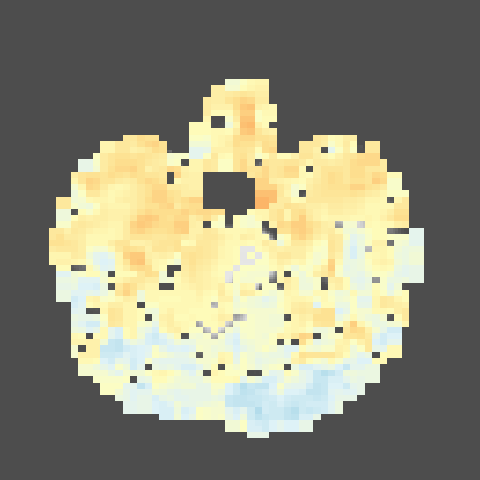
\includegraphics[width=0.16\linewidth]{cor-axial-age-mW} &
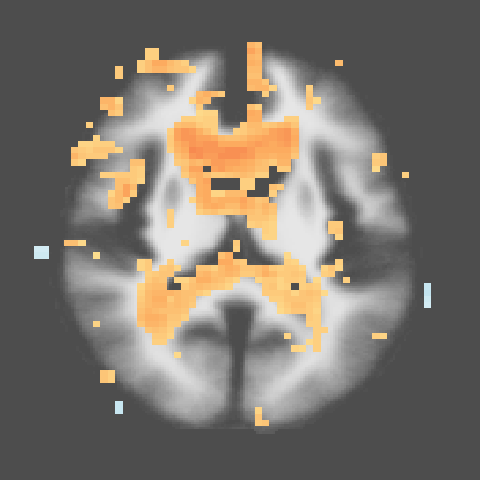
\includegraphics[width=0.16\linewidth]{cor-axial-age-t-mW} &

\includegraphics[width=0.16\linewidth]{cor-axial-cdr-mW} &

\includegraphics[width=0.16\linewidth]{cor-axial-cdr-t-mW} &
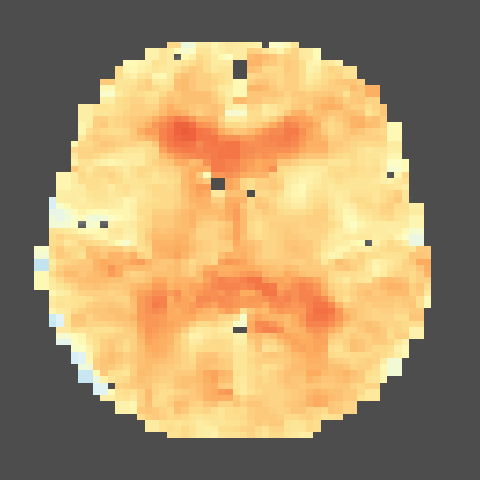
\includegraphics[width=0.16\linewidth]{cor-axial-mmse-mW} &

\includegraphics[width=0.16\linewidth]{cor-axial-mmse-t-mW} \\ 
%
        &

\includegraphics[width=0.16\linewidth]{cor-coronal-age-mW} &
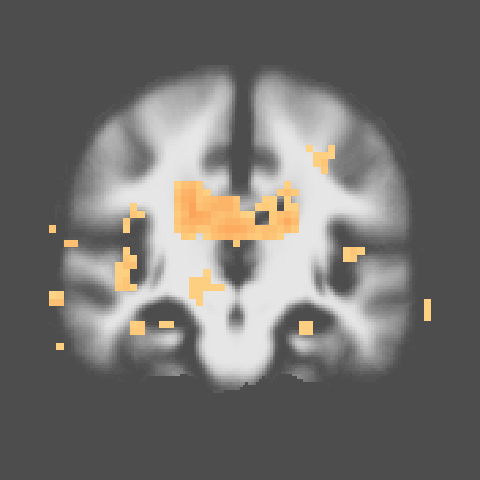
\includegraphics[width=0.16\linewidth]{cor-coronal-age-t-mW} &

\includegraphics[width=0.16\linewidth]{cor-coronal-cdr-mW} &

\includegraphics[width=0.16\linewidth]{cor-coronal-cdr-t-mW} &

\includegraphics[width=0.16\linewidth]{cor-coronal-mmse-mW} &
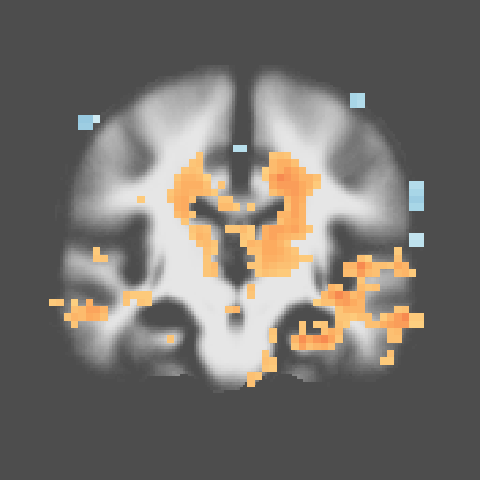
\includegraphics[width=0.16\linewidth]{cor-coronal-mmse-t-mW} \\ 
%
        &
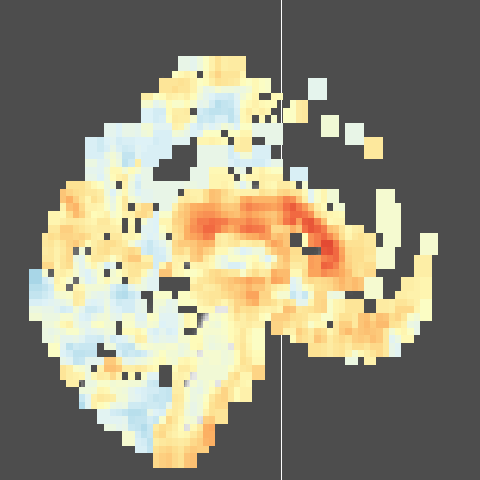
\includegraphics[width=0.16\linewidth]{cor-sagital-age-mW} &
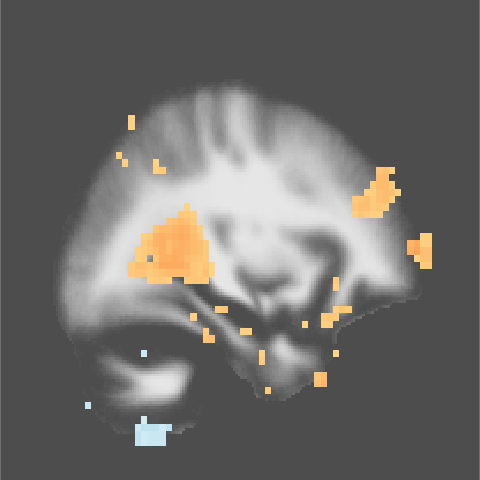
\includegraphics[width=0.16\linewidth]{cor-sagital-age-t-mW} &
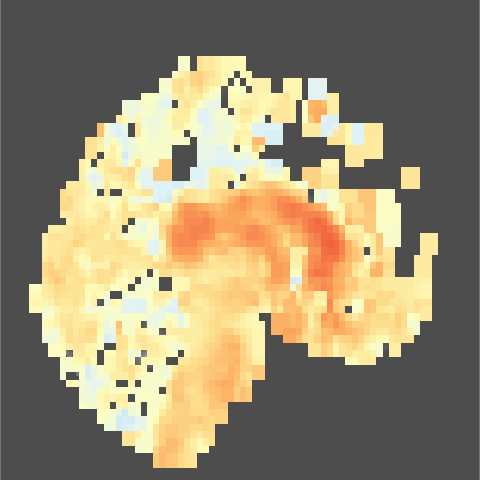
\includegraphics[width=0.16\linewidth]{cor-sagital-cdr-mW} &
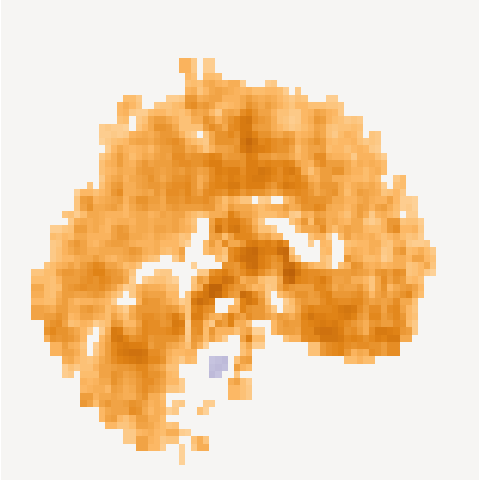
\includegraphics[width=0.16\linewidth]{cor-sagital-cdr-t-mW} &
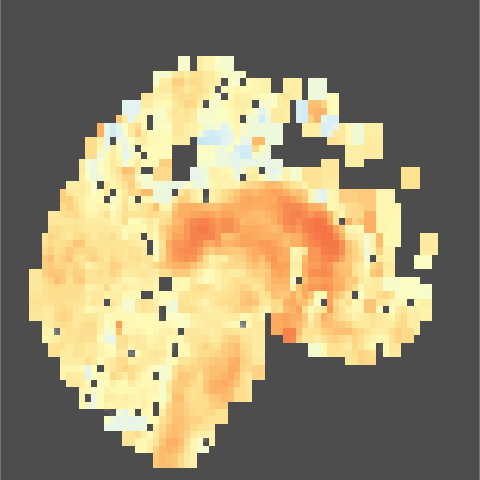
\includegraphics[width=0.16\linewidth]{cor-sagital-mmse-mW} &
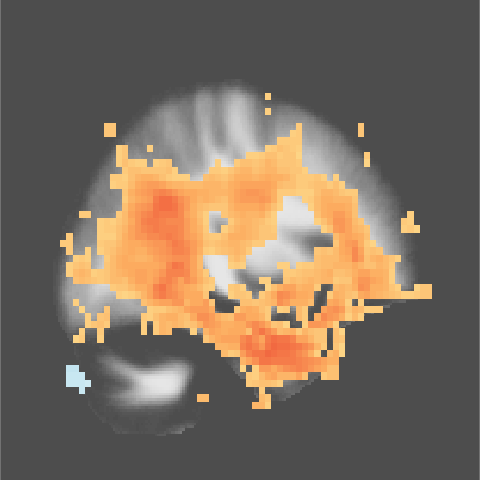
\includegraphics[width=0.16\linewidth]{cor-sagital-mmse-t-mW} \\ \hline \hline
%
\parbox[t]{2mm}{\multirow{3}{*}{\rotatebox[origin=c]{90}{Transport Cost}}}&

\includegraphics[width=0.16\linewidth]{cor-axial-age-tW} &
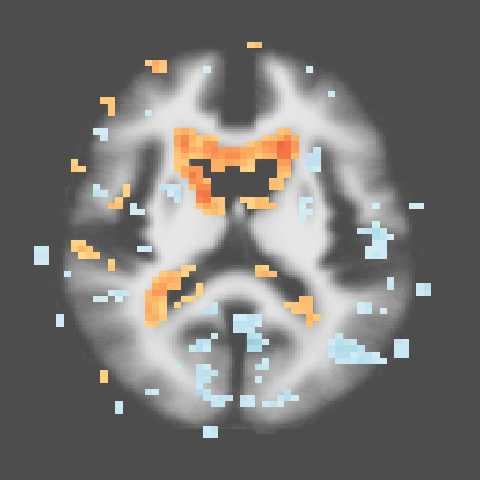
\includegraphics[width=0.16\linewidth]{cor-axial-age-t-tW} &

\includegraphics[width=0.16\linewidth]{cor-axial-cdr-tW} &

\includegraphics[width=0.16\linewidth]{cor-axial-cdr-t-tW} &

\includegraphics[width=0.16\linewidth]{cor-axial-mmse-tW} &
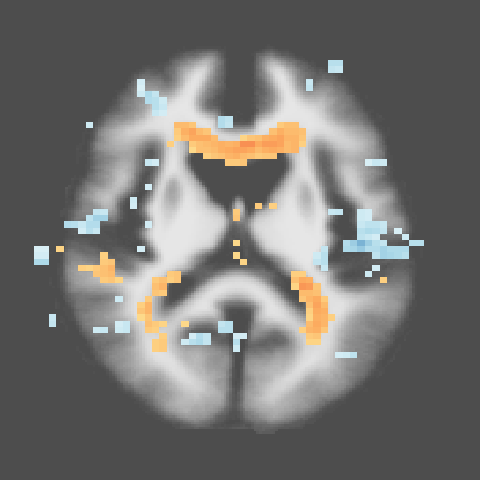
\includegraphics[width=0.16\linewidth]{cor-axial-mmse-t-tW} \\ 
%
        &

\includegraphics[width=0.16\linewidth]{cor-coronal-age-tW} &
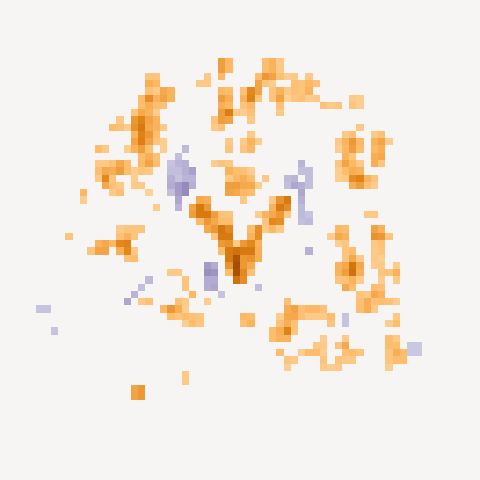
\includegraphics[width=0.16\linewidth]{cor-coronal-age-t-tW} &

\includegraphics[width=0.16\linewidth]{cor-coronal-cdr-tW} &
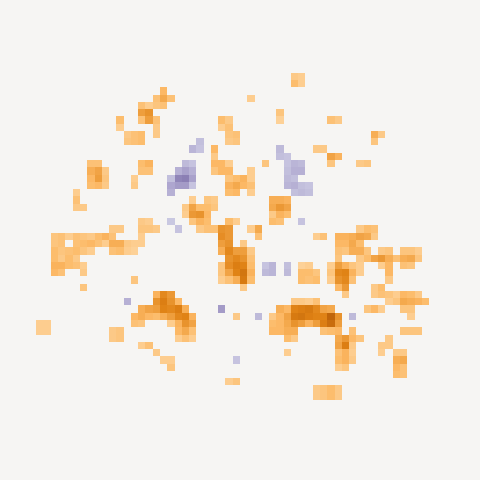
\includegraphics[width=0.16\linewidth]{cor-coronal-cdr-t-tW} &
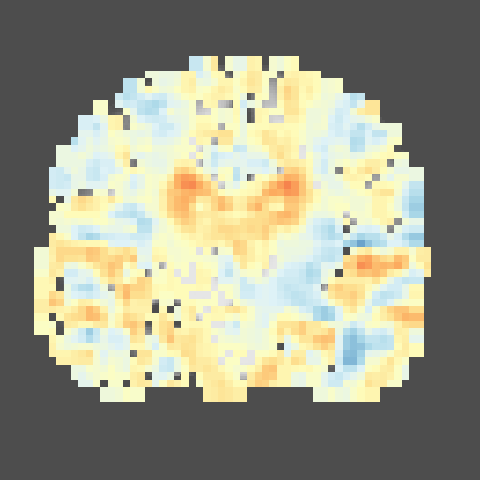
\includegraphics[width=0.16\linewidth]{cor-coronal-mmse-tW} &
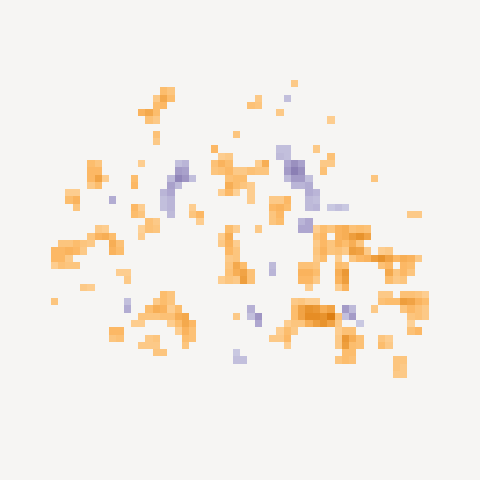
\includegraphics[width=0.16\linewidth]{cor-coronal-mmse-t-tW} \\ 
%
        &
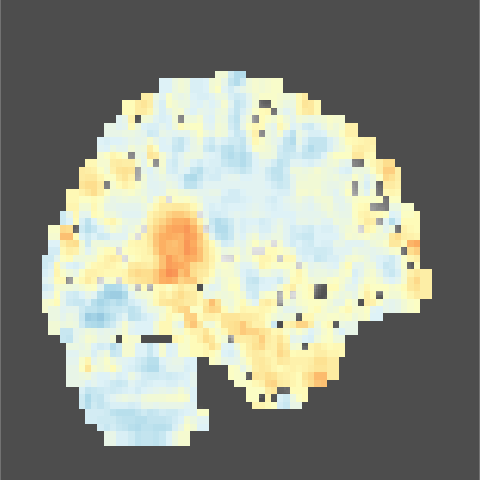
\includegraphics[width=0.16\linewidth]{cor-sagital-age-tW} &
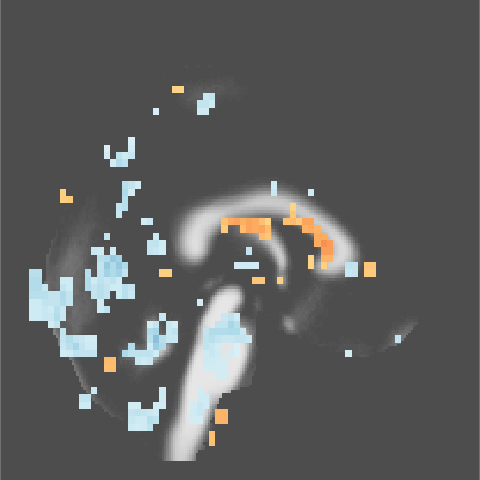
\includegraphics[width=0.16\linewidth]{cor-sagital-age-t-tW} &
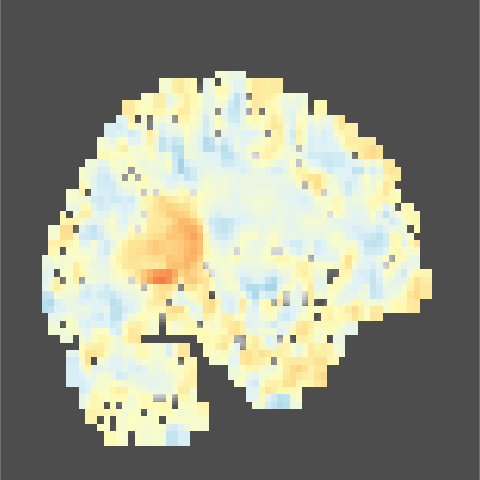
\includegraphics[width=0.16\linewidth]{cor-sagital-cdr-tW} &
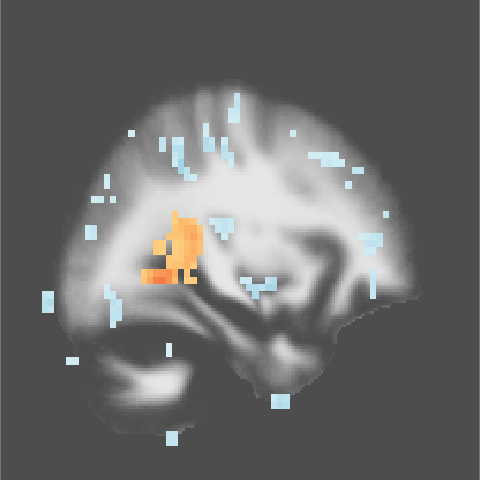
\includegraphics[width=0.16\linewidth]{cor-sagital-cdr-t-tW} &
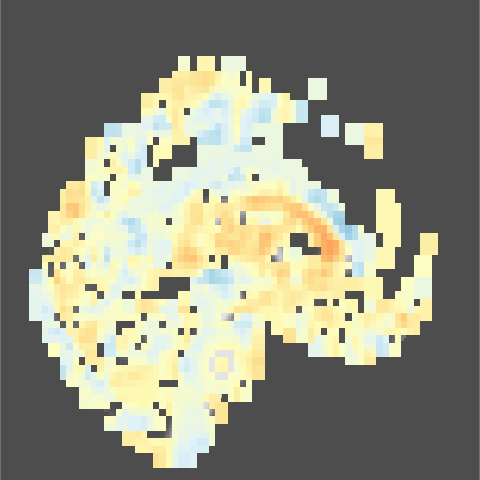
\includegraphics[width=0.16\linewidth]{cor-sagital-mmse-tW} &
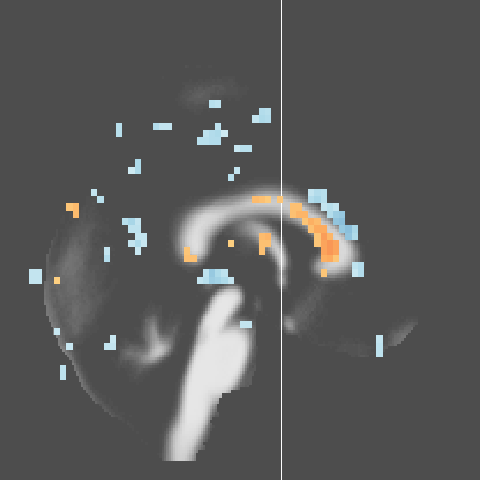
\includegraphics[width=0.16\linewidth]{cor-sagital-mmse-t-tW} \\ \hline \hline
%
& \parbox[b][4mm]{6mm}{Age} 
& \parbox[b][4mm]{6mm}{Age\textsuperscript{*}} 
& \parbox[b][4mm]{6mm}{CDR} 
& \parbox[b][4mm]{6mm}{CDR\textsuperscript{*}}
& \parbox[b][4mm]{6mm}{MMSE}
& \parbox[b][4mm]{6mm}{MMSE\textsuperscript{*}}
\end{tabular}
\caption{\label{fig:cor-oasis-gray}
Correlation of age, MMSE and CDR with optimal transport mass imbalances and
optimal transport costs of gray matter. The columns with a \textsuperscript{*}
only show the voxels were the correlation has a permutation tested p-value less
than 0.05  }
\end{figure}
\endgroup

\begingroup
\renewcommand{\arraystretch}{0}
\setlength{\tabcolsep}{0pt}
\begin{figure}[bth]
\centering
\begin{tabular}{l|cc|cc|cc}
\parbox[t]{4mm}{\multirow{3}{*}{\rotatebox[origin=c]{90}{Mass Imbalance}}}&
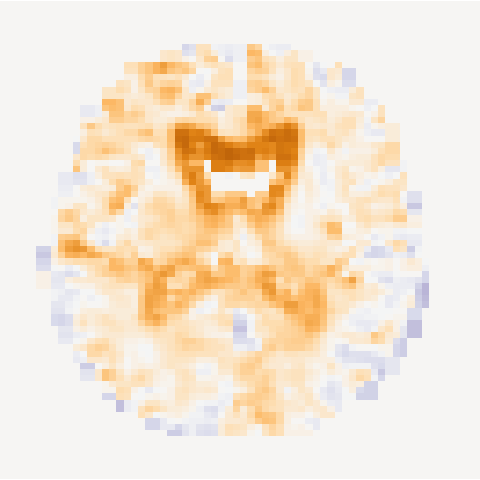
\includegraphics[width=0.16\linewidth]{cor-axial-age-mG} &

\includegraphics[width=0.16\linewidth]{cor-axial-age-t-mG} &
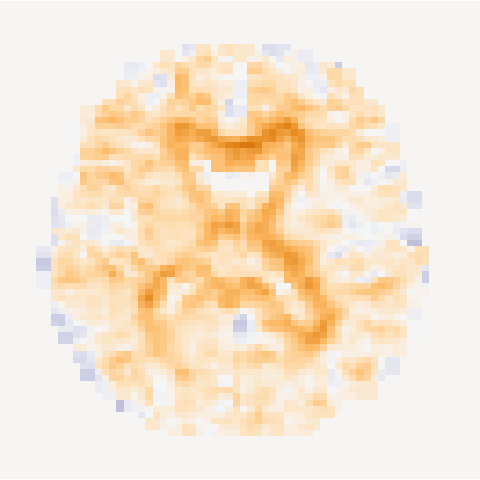
\includegraphics[width=0.16\linewidth]{cor-axial-cdr-mG} &

\includegraphics[width=0.16\linewidth]{cor-axial-cdr-t-mG} &
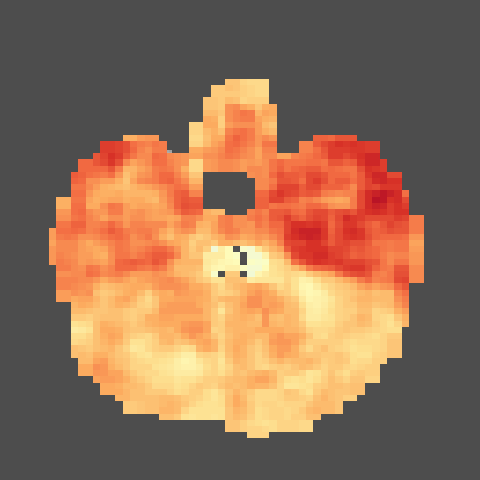
\includegraphics[width=0.16\linewidth]{cor-axial-mmse-mG} &

\includegraphics[width=0.16\linewidth]{cor-axial-mmse-t-mG} \\ 
%
        &

\includegraphics[width=0.16\linewidth]{cor-coronal-age-mG} &

\includegraphics[width=0.16\linewidth]{cor-coronal-age-t-mG} &
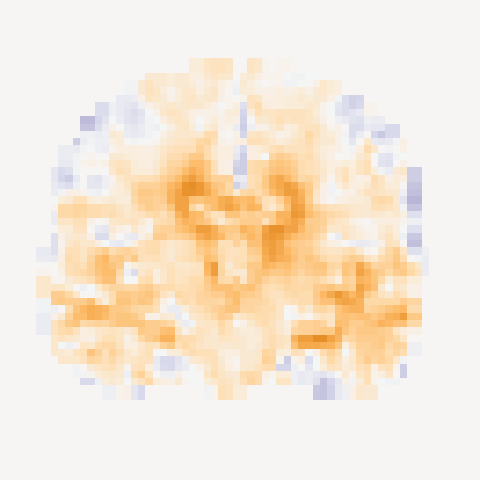
\includegraphics[width=0.16\linewidth]{cor-coronal-cdr-mG} &

\includegraphics[width=0.16\linewidth]{cor-coronal-cdr-t-mG} &

\includegraphics[width=0.16\linewidth]{cor-coronal-mmse-mG} &

\includegraphics[width=0.16\linewidth]{cor-coronal-mmse-t-mG} \\ 
%
        &
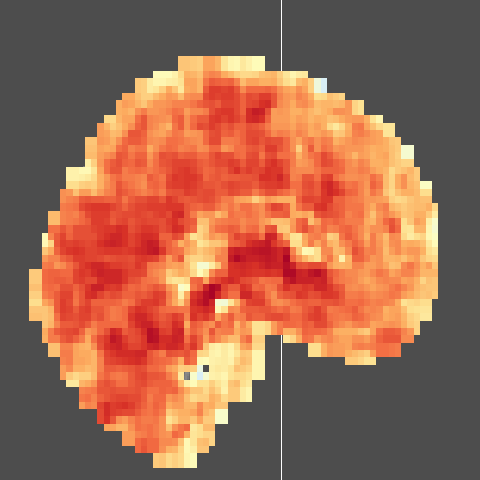
\includegraphics[width=0.16\linewidth]{cor-sagital-age-mG} &
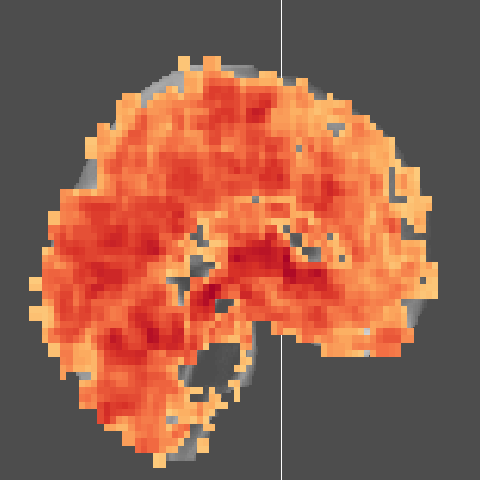
\includegraphics[width=0.16\linewidth]{cor-sagital-age-t-mG} &
\includegraphics[width=0.16\linewidth]{cor-sagital-cdr-mG} &
\includegraphics[width=0.16\linewidth]{cor-sagital-cdr-t-mG} &
\includegraphics[width=0.16\linewidth]{cor-sagital-mmse-mG} &
\includegraphics[width=0.16\linewidth]{cor-sagital-mmse-t-mG} \\ \hline \hline
%
\parbox[t]{2mm}{\multirow{3}{*}{\rotatebox[origin=c]{90}{Transport Cost}}}&
\includegraphics[width=0.16\linewidth]{cor-axial-age-tG} &
\includegraphics[width=0.16\linewidth]{cor-axial-age-t-tG} &
\includegraphics[width=0.16\linewidth]{cor-axial-cdr-tG} &
\includegraphics[width=0.16\linewidth]{cor-axial-cdr-t-tG} &
\includegraphics[width=0.16\linewidth]{cor-axial-mmse-tG} &
\includegraphics[width=0.16\linewidth]{cor-axial-mmse-t-tG} \\ 
%
        &
\includegraphics[width=0.16\linewidth]{cor-coronal-age-tG} &
\includegraphics[width=0.16\linewidth]{cor-coronal-age-t-tG} &
\includegraphics[width=0.16\linewidth]{cor-coronal-cdr-tG} &
\includegraphics[width=0.16\linewidth]{cor-coronal-cdr-t-tG} &
\includegraphics[width=0.16\linewidth]{cor-coronal-mmse-tG} &
\includegraphics[width=0.16\linewidth]{cor-coronal-mmse-t-tG} \\ 
%
        &
\includegraphics[width=0.16\linewidth]{cor-sagital-age-tG} &
\includegraphics[width=0.16\linewidth]{cor-sagital-age-t-tG} &
\includegraphics[width=0.16\linewidth]{cor-sagital-cdr-tG} &
\includegraphics[width=0.16\linewidth]{cor-sagital-cdr-t-tG} &
\includegraphics[width=0.16\linewidth]{cor-sagital-mmse-tG} &
\includegraphics[width=0.16\linewidth]{cor-sagital-mmse-t-tG} \\ \hline \hline
%%
& \parbox[b][4mm]{6mm}{Age} 
& \parbox[b][4mm]{6mm}{Age\textsuperscript{*}} 
& \parbox[b][4mm]{6mm}{CDR} 
& \parbox[b][4mm]{6mm}{CDR\textsuperscript{*}}
& \parbox[b][4mm]{6mm}{MMSE}
& \parbox[b][4mm]{6mm}{MMSE\textsuperscript{*}}
\end{tabular}
\caption{\label{fig:cor-oasis-white}
Correlation of age, MMSE and CDR with optimal transport mass imbalances and
optimal transport costs of white matter. The columns with a \textsuperscript{*}
only show the voxels were the correlation has a permutation tested p-value less
than 0.05  }
\end{figure}
\endgroup


%%%VBM glmnet /linear models




%%%%Optimal transport glmnet / linear models
> build.linear.model( age[age.index], all[age.index,ind$non.zero])$anova
Analysis of Variance Table

Response: y
           Df  Sum Sq Mean Sq F value    Pr(>F)    
mG.35390    1  452.79  452.79 48.6765 2.537e-10 ***
mG.47319    1  397.31  397.31 42.7120 2.155e-09 ***
mW.10288    1  608.08  608.08 65.3711 9.769e-13 ***
mW.32409    1  380.72  380.72 40.9285 4.158e-09 ***
mW.34788    1   11.55   11.55  1.2421 0.2675328    
mW.35355    1  107.21  107.21 11.5259 0.0009610 ***
mW.41736    1   27.60   27.60  2.9667 0.0878573 .  
mW.44233    1   60.30   60.30  6.4829 0.0123018 *  
mW.44276    1   44.15   44.15  4.7463 0.0315351 *  
mW.46565    1   13.08   13.08  1.4064 0.2382650    
mW.46653    1   10.66   10.66  1.1456 0.2868669    
mW.47145    1   15.81   15.81  1.6996 0.1951067    
mW.58048    1    2.13    2.13  0.2292 0.6330675    
mW.58092    1    6.07    6.07  0.6530 0.4208182    
mW.58137    1   14.06   14.06  1.5119 0.2215200    
mW.81162    1   58.13   58.13  6.2494 0.0139274 *  
mW.81206    1    1.86    1.86  0.2000 0.6556251    
mW.83581    1    4.67    4.67  0.5018 0.4802432    
tG.5201     1  120.23  120.23 12.9254 0.0004902 ***
tG.15161    1   88.43   88.43  9.5064 0.0025995 ** 
tG.35152    1  120.20  120.20 12.9218 0.0004910 ***
tG.56970    1  140.95  140.95 15.1531 0.0001719 ***
tG.57013    1   73.48   73.48  7.8989 0.0058745 ** 
tG.60180    1   12.94   12.94  1.3910 0.2408212    
tw.49347    1   59.03   59.03  6.3455 0.0132328 *  
tw.51634    1   19.76   19.76  2.1241 0.1478975    
tw.55270    1    8.28    8.28  0.8897 0.3476540    
tw.83450    1   33.18   33.18  3.5672 0.0616126 .  
Residuals 108 1004.61    9.30                      
---
Signif. codes:  0 ‘***’ 0.001 ‘**’ 0.01 ‘*’ 0.05 ‘.’ 0.1 ‘ ’ 1
> summary(  build.linear.model( age[age.index], all[age.index,ind$non.zero])$lm )

Call:
lm(formula = y ~ ., data = data.frame(y = y, x))

Residuals:
    Min      1Q  Median      3Q     Max 
-7.2959 -1.6669  0.0181  1.5565  7.6762 

Coefficients:
              Estimate Std. Error t value Pr(>|t|)    
(Intercept)  7.645e+01  9.753e-01  78.391   <2e-16 ***
mG.35390    -3.474e-01  1.430e-01  -2.430   0.0168 *  
mG.47319    -1.606e-02  1.536e-01  -0.105   0.9169    
mW.10288    -9.264e+05  5.529e+05  -1.676   0.0967 .  
mW.32409    -1.143e-01  1.326e-01  -0.862   0.3905    
mW.34788     1.261e-01  1.675e-01   0.753   0.4534    
mW.35355    -2.656e-01  2.164e-01  -1.227   0.2224    
mW.41736    -5.270e-02  7.319e-02  -0.720   0.4731    
mW.44233     2.144e-01  3.346e-01   0.641   0.5230    
mW.44276    -1.938e-01  2.383e-01  -0.813   0.4178    
mW.46565    -2.752e-01  4.190e-01  -0.657   0.5127    
mW.46653     8.739e-02  2.716e-01   0.322   0.7483    
mW.47145    -2.127e-02  1.377e-01  -0.154   0.8775    
mW.58048    -4.132e-02  2.625e-01  -0.157   0.8752    
mW.58092    -4.960e-02  3.270e-01  -0.152   0.8797    
mW.58137    -6.686e-02  2.454e-01  -0.272   0.7858    
mW.81162    -1.355e-01  2.790e-01  -0.486   0.6283    
mW.81206     1.095e-01  3.178e-01   0.345   0.7310    
mW.83581    -1.362e-01  1.510e-01  -0.902   0.3690    
tG.5201      1.367e+00  7.404e-01   1.846   0.0676 .  
tG.15161     2.641e-01  1.097e-01   2.409   0.0177 *  
tG.35152     8.047e-02  3.093e-02   2.602   0.0106 *  
tG.56970    -4.579e+02  3.260e+02  -1.404   0.1631    
tG.57013    -1.873e+03  9.301e+02  -2.014   0.0465 *  
tG.60180     5.572e-04  4.735e-04   1.177   0.2419    
tw.49347    -1.140e-04  1.256e-03  -0.091   0.9279    
tw.51634    -1.563e-03  1.454e-03  -1.075   0.2846    
tw.55270     1.488e+03  2.232e+03   0.667   0.5062    
tw.83450    -8.596e-04  4.551e-04  -1.889   0.0616 .  
---
Signif. codes:  0 ‘***’ 0.001 ‘**’ 0.01 ‘*’ 0.05 ‘.’ 0.1 ‘ ’ 1

Residual standard error: 3.05 on 108 degrees of freedom
Multiple R-squared:  0.7422,	Adjusted R-squared:  0.6754 
F-statistic: 11.11 on 28 and 108 DF,  p-value: < 2.2e-16

>


> build.linear.model( cdr[cdr.index], all[cdr.index,ind$non.zero])$anova
Analysis of Variance Table

Response: y
           Df Sum Sq Mean Sq F value    Pr(>F)    
mW.15261    1 4.7664  4.7664 68.3471 2.696e-13 ***
mW.19740    1 1.0071  1.0071 14.4415 0.0002328 ***
mW.26275    1 0.8482  0.8482 12.1622 0.0006917 ***
mW.26515    1 0.4747  0.4747  6.8069 0.0102870 *  
mW.26516    1 0.0003  0.0003  0.0040 0.9499686    
mW.28759    1 0.0401  0.0401  0.5746 0.4499910    
mW.28803    1 0.0504  0.0504  0.7226 0.3970552    
mW.28986    1 0.0124  0.0124  0.1783 0.6736484    
mW.30919    1 0.0320  0.0320  0.4590 0.4994502    
mW.31047    1 0.0087  0.0087  0.1242 0.7251502    
mW.37502    1 0.1681  0.1681  2.4109 0.1232374    
mW.46809    1 0.1013  0.1013  1.4524 0.2306223    
tG.508      1 0.9945  0.9945 14.2599 0.0002537 ***
tG.552      1 0.0207  0.0207  0.2974 0.5865795    
tG.2841     1 0.0599  0.0599  0.8585 0.3561025    
tG.2884     1 0.1344  0.1344  1.9275 0.1677143    
tG.21905    1 1.7449  1.7449 25.0202 2.056e-06 ***
tG.69510    1 1.1820  1.1820 16.9495 7.255e-05 ***
tw.35578    1 0.3562  0.3562  5.1077 0.0257018 *  
tw.46838    1 0.1289  0.1289  1.8488 0.1765849    
tw.66592    1 0.2250  0.2250  3.2260 0.0751026 .  
Residuals 115 8.0198  0.0697                      
---
Signif. codes:  0 ‘***’ 0.001 ‘**’ 0.01 ‘*’ 0.05 ‘.’ 0.1 ‘ ’ 1
> summary(  build.linear.model( cdr[cdr.index], all[cdr.index,ind$non.zero])$lm )

Call:
lm(formula = y ~ ., data = data.frame(y = y, x))

Residuals:
     Min       1Q   Median       3Q      Max 
-0.49165 -0.15764  0.00573  0.13733  1.13225 

Coefficients:
              Estimate Std. Error t value Pr(>|t|)    
(Intercept)  5.039e-01  8.995e-02   5.602 1.47e-07 ***
mW.15261    -3.043e+03  2.178e+03  -1.397 0.165146    
mW.19740    -1.404e-02  2.376e-02  -0.591 0.555772    
mW.26275    -1.063e-02  1.195e-02  -0.890 0.375436    
mW.26515    -3.440e-02  5.217e-02  -0.660 0.510888    
mW.26516     2.313e-02  3.792e-02   0.610 0.543112    
mW.28759    -4.882e-02  3.116e-02  -1.567 0.119907    
mW.28803     1.065e-02  3.471e-02   0.307 0.759562    
mW.28986    -3.702e-03  1.133e-02  -0.327 0.744475    
mW.30919    -3.991e-03  1.053e-02  -0.379 0.705334    
mW.31047     5.306e-02  3.278e-02   1.619 0.108224    
mW.37502    -1.261e-02  9.434e-03  -1.337 0.183833    
mW.46809    -3.850e-03  5.822e-03  -0.661 0.509711    
tG.508      -1.043e+01  1.576e+01  -0.662 0.509257    
tG.552       1.440e+00  1.594e+00   0.903 0.368227    
tG.2841      2.244e-02  1.600e-02   1.402 0.163673    
tG.2884     -1.345e-02  1.155e-02  -1.165 0.246621    
tG.21905     2.542e-03  7.543e-04   3.369 0.001026 ** 
tG.69510     3.096e-04  8.019e-05   3.860 0.000187 ***
tw.35578    -7.095e-05  7.569e-05  -0.937 0.350531    
tw.46838    -6.802e-05  6.278e-05  -1.083 0.280920    
tw.66592    -1.013e-01  5.640e-02  -1.796 0.075103 .  
---
Signif. codes:  0 ‘***’ 0.001 ‘**’ 0.01 ‘*’ 0.05 ‘.’ 0.1 ‘ ’ 1

Residual standard error: 0.2641 on 115 degrees of freedom
Multiple R-squared:  0.6064,	Adjusted R-squared:  0.5345 
F-statistic: 8.437 on 21 and 115 DF,  p-value: 5.228e-15

> 



  build.linear.model( mmse[mmse.index], all[mmse.index,ind$non.zero])$anova 
Analysis of Variance Table

Response: y
           Df  Sum Sq Mean Sq F value    Pr(>F)    
mW.14977    1  374.49  374.49 42.4923 1.578e-09 ***
mW.28802    1   92.72   92.72 10.5208  0.001514 ** 
mW.28803    1    4.47    4.47  0.5073  0.477654    
mW.28986    1   33.64   33.64  3.8173  0.052959 .  
mW.35808    1   11.54   11.54  1.3093  0.254716    
mW.42139    1   17.54   17.54  1.9897  0.160853    
mW.46853    1   20.00   20.00  2.2689  0.134513    
tG.509      1  149.53  149.53 16.9667 6.868e-05 ***
tG.54723    1  171.01  171.01 19.4037 2.249e-05 ***
tG.78265    1  147.69  147.69 16.7577 7.567e-05 ***
tw.49090    1   59.98   59.98  6.8054  0.010196 *  
Residuals 125 1101.63    8.81                      
---
Signif. codes:  0 ‘***’ 0.001 ‘**’ 0.01 ‘*’ 0.05 ‘.’ 0.1 ‘ ’ 1
> summary(  build.linear.model( mmse[mmse.index], all[mmse.index,ind$non.zero])$lm )

Call:
lm(formula = y ~ ., data = data.frame(y = y, x))

Residuals:
     Min       1Q   Median       3Q      Max 
-10.6100  -1.4960   0.4654   2.1175   5.2417 

Coefficients:
              Estimate Std. Error t value Pr(>|t|)    
(Intercept)  2.455e+01  6.280e-01  39.087  < 2e-16 ***
mW.14977     2.908e+00  2.157e+00   1.348 0.180084    
mW.28802     1.457e-01  2.909e-01   0.501 0.617253    
mW.28803    -1.121e-01  2.942e-01  -0.381 0.703862    
mW.28986     1.236e-01  1.462e-01   0.845 0.399634    
mW.35808     1.335e-02  1.730e-01   0.077 0.938631    
mW.42139     3.368e-03  1.333e-01   0.025 0.979882    
mW.46853     5.715e-02  6.197e-02   0.922 0.358186    
tG.509      -1.902e+01  8.063e+00  -2.359 0.019872 *  
tG.54723    -1.368e+01  3.580e+00  -3.823 0.000207 ***
tG.78265    -9.828e+02  2.409e+02  -4.079    8e-05 ***
tw.49090     8.518e-04  3.265e-04   2.609 0.010196 *  
---
Signif. codes:  0 ‘***’ 0.001 ‘**’ 0.01 ‘*’ 0.05 ‘.’ 0.1 ‘ ’ 1

Residual standard error: 2.969 on 125 degrees of freedom
Multiple R-squared:  0.4956,	Adjusted R-squared:  0.4513 
F-statistic: 11.17 on 11 and 125 DF,  p-value: 3.371e-14


